\documentclass{article}
\usepackage[utf8]{inputenc}

\title{\begin{center}
\Large
\textbf{
    Transmit Beamforming \linebreak And Application in Massive MIMO
    }
\end{center}}
\author{Jinkun Zhang , April 2018}
%\date{April 2018}
\date{}

\usepackage{natbib}
\usepackage{geometry}
\usepackage{graphicx}
\geometry{left=1.5cm,right=1.5cm,top=1.5cm,bottom=2cm}

\begin{document}

\twocolumn
\maketitle
\section{Introduction}

Beamforming, or known as spatial filtering, is a signal processing technique used in antenna arrays for directional signal transmission or reception. Beamforming can be used at both the transmitting and receiving ends in order to achieve spatial selectivity.\cite{BeamformingBook}

Massive multiple-input multiple-output (MIMO) system, or called large-scale MIMO system, is an arrangement of multiple-user MIMO systems (MU-MIMO) wherein large quantities of antenna elements at base station (BS) and large quantities of antennas at terminals are deployed.\cite{MassiveMIMO}

Massive MIMO system can improve the capacity of wireless communication system efficiently, due to a large number of channels implemented. However, using a large amount of antennas may causes interference problems, which can be mitigated by deploying beamforming antennas instead of conventional antennas.

\begin{figure}[b!]
\centering
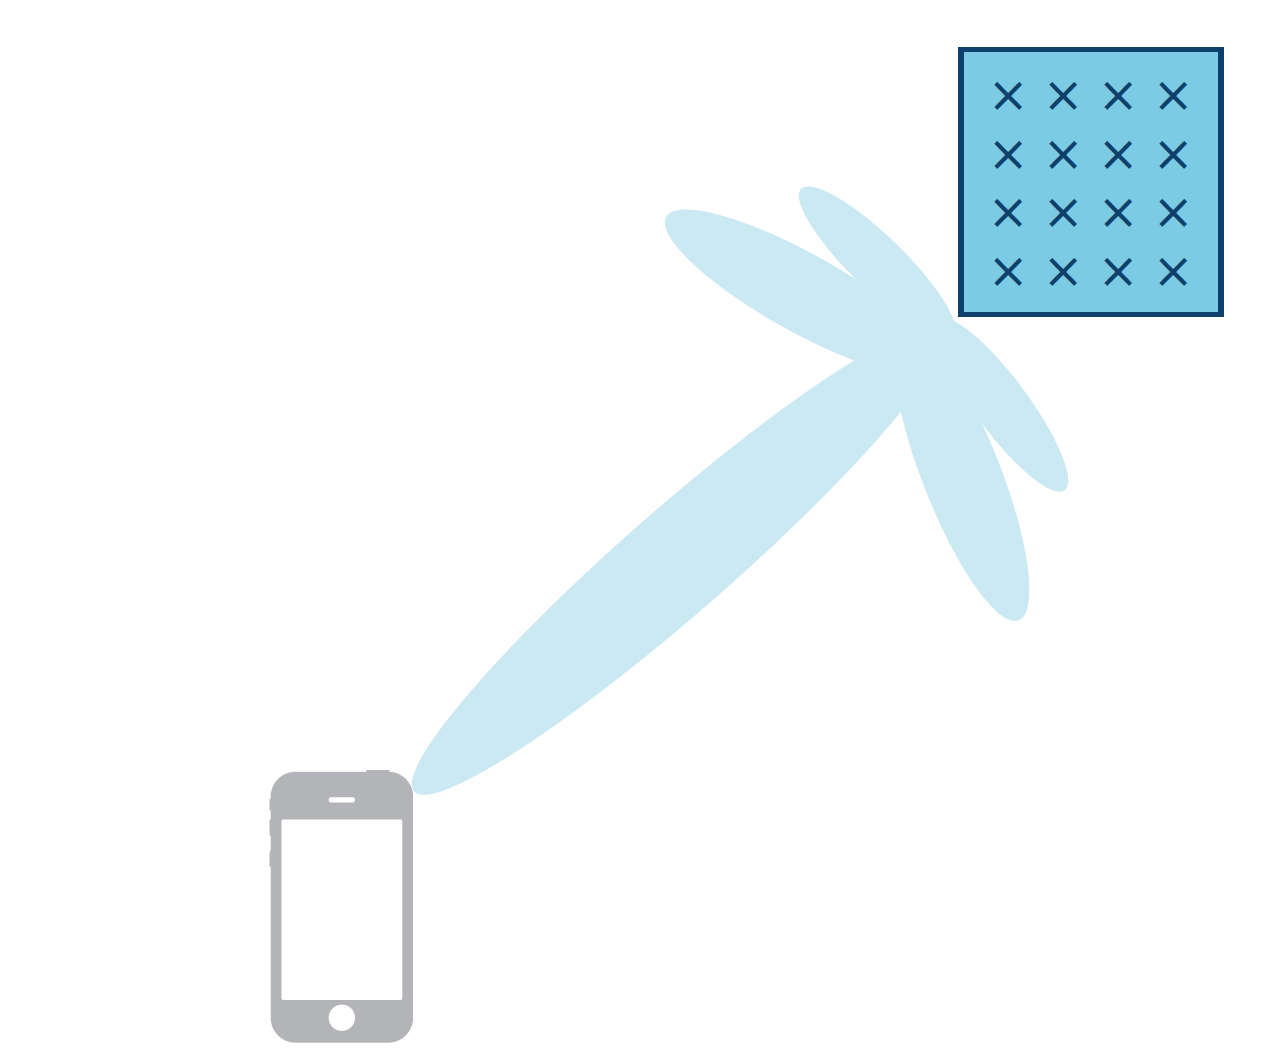
\includegraphics[scale=0.2]{beamforming2.png}
\caption{Beamforming}
\label{fig:beamforming}
\end{figure}

\begin{figure}[b!]
\centering
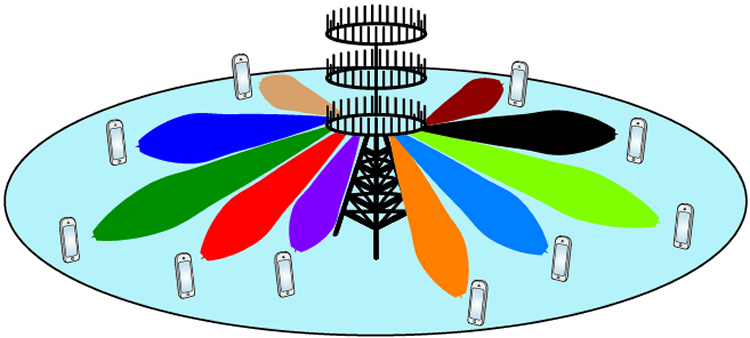
\includegraphics[scale=0.35]{massive-mimo.jpg}
\caption{Multi-user Massive MIMO with Beamforming}
\label{fig:massivemimo}
\end{figure}


\section{Transmit Beamforming Technique}
Transmit beamforming, or TxBF, can improve considerably the performance of MIMO system. The objective of transmit beamforming is to maximise each user's received signal power while minimising the interference signal power from other users, hence increasing capacity. This can be achieved by transmitting the same signal from all transmitters with different amplitudes and phases. These multiple versions of the transmitted signal will pass through different MIMO channels such they are added constructively at the desired user and destructively at other users.\cite{BeamformingFuture}
As a simple case, the linear equally spaced (LES) array is considered suitable for a basic beamforming configuration implementation.

Beamforming is widely used in millimeter wave multiple user communication system study. In transmitter side, there're two kinds of beamforming, namely analog beamforming and digital beamforming. Meanwhile, Beamforming method can be divided into two approaches, namely switched array beamforming, which is aimed to a situation with predefined beams, and adaptive array beamforming, which assumes that the BS modernizes the localization of the mobile station.

\begin{figure}[h!]
\centering
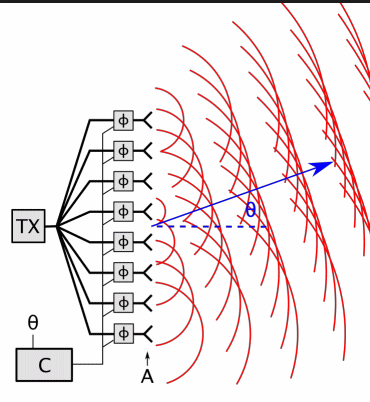
\includegraphics[scale=0.4]{beamforming.png}
\caption{Transmit Beamforming on LES Array}
\label{fig:beamformingLES}
\end{figure}

\begin{figure}[h!]
\centering
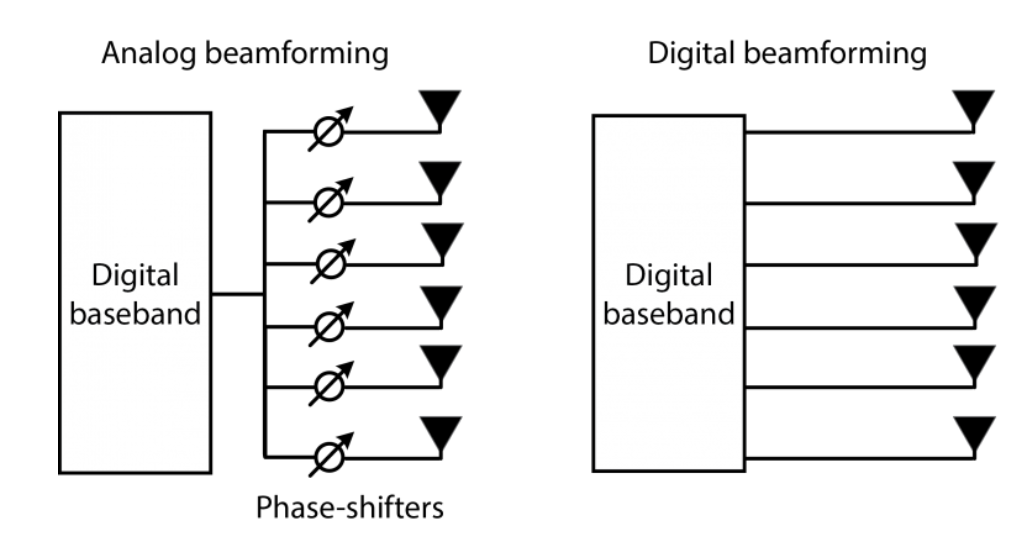
\includegraphics[scale=0.3]{twobeamforming.png}
\caption{Structure of Analog and Digital Beamforming}
\label{fig:Twobeamforming}
\end{figure}

\section{Application in Massive MIMO}
Millimeter wave has been widely studied and considered the core part of next generation communication systems. Millimeter wave has some features differing from conventional carry frequency, such as high pass loss with time varying small scale fading, and significant directionality\cite{mmWave}.
These features makes millimeter wave suitable for reducing the inter-user beamforming interference, thus suitable for massive MIMO system.

In conventional SISO or small scale MIMO system, one of the main impairments in wireless communications is small-scale channel fading. This refers to random fluctuations in the channel gain, which are caused by microscopic changes in the propagation environments. However, in massive MIMO, channel hardening is taking place, where channel hardening means that, with a large amount of MIMO antennas, due to central limit theorem, a fading channel behaves as if it was a non-fading channel, namely the variance of ratio $ \frac{\|h^2\|}{E\{\|h^2\|\}} $ is decreasing rapidly with the increase of number of antennas, where $h$ is the channel vector. This feature is firstly studied in \cite{ChannelHarden}.

\begin{figure}[h!]
\centering
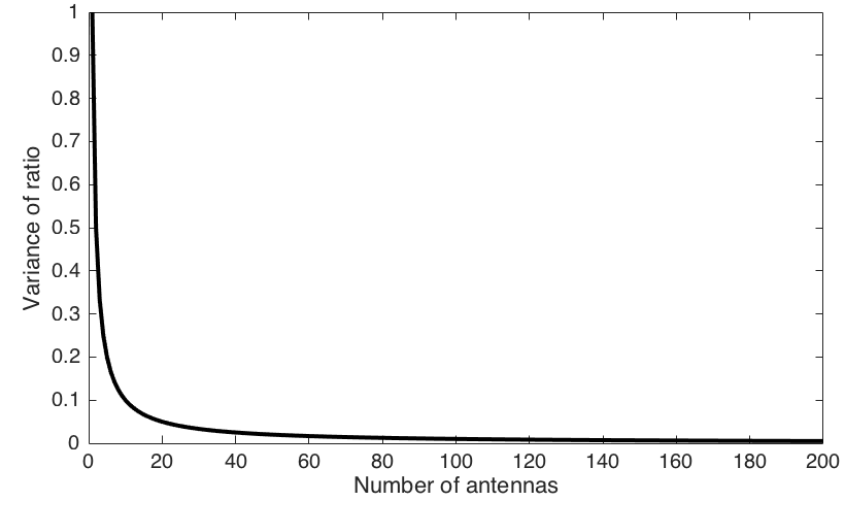
\includegraphics[scale=0.4]{channelharden.png}
\caption{Channel Hardening in Rayleigh Channel}
\label{fig:channelharden}
\end{figure}

Extensive work is currently being done by researchers to develop an inclusive statistical mm-wave propagation model for channel modelling in massive MIMO that can help estimate the channel state information (CSI), which is important in transmit beamforming.

Additionally, it will be extremely expensive and complex to address digital beamforming with the implementation of large numbers of antennas. Therefore, addressing hybrid beamforming approaches, which are combinations of digital beamforming and analogue beamforming, as shown in \cite{mmWaveandMIMO}, promises to provide enhancements in terms of both power consumption and performance.

\section{Issues and Future Trends }
By\cite{BeamformingFuture},
there are several issues that
have received considerable attention in recent years
and must be addressed before implementing massive
MIMO systems in practice:


\begin{itemize}

\item[-] Pilot contamination

\item[-] Millimetre-wave hybrid beamforming

\item[-] Channel correlation of beamforming array
antennas for millimetre-waves

\item[-] Sparsity of beams
\item[-] Beamforming localization for massive MIMO
systems

\end{itemize}

\section{Conclusion}
Massive multiple-input multiple-output (MIMO) systems combined with beamforming antenna array technologies are
expected to play a key role in next-generation wireless communication systems.
This paper briefly discuss both the fundamental theory and the state-of-the-art research on types of beamforming techniques that can be deployed in massive MIMO systems and to clarify the importance of beamforming techniques in massive
MIMO systems for eliminating and resolving the many technical hitches that massive MIMO system implementation faces.
To overcome the limitations, a combination of analog and digital beamforming
technique that can provide better performance in massive MIMO systems, satisfies the requirements of next-generation
wireless communication systems.

\bibliographystyle{unsrt}
\bibliography{references}
\end{document}
